\documentclass[a4paper]{article}
%%%%%%%%%%%%%%%%%%%%%%%%%%%%%%%%%%%%%%%%%%%%%%%%%%%%%%%%%%%
\usepackage[utf8]{inputenc}
\usepackage[english]{babel}
\usepackage{url}
\usepackage{natbib}
\usepackage{xspace}
\usepackage{graphicx}
\usepackage{graphicx}
\usepackage{caption}
\usepackage{subcaption}
\usepackage{manifest}
\usepackage{listings}
\usepackage{amsfonts}
\usepackage{amsmath}
\usepackage{algorithm}
\usepackage{algorithmic}
\usepackage{appendix}
\usepackage{color}
\usepackage{listings}
\usepackage[pdftex,bookmarks,colorlinks,pdfauthor={Luca Mella},pdftitle={Report-SMA1213}, pdftex]{hyperref}

\definecolor{mygreen}{rgb}{0,0.6,0}
\definecolor{mygray}{rgb}{0.5,0.5,0.5}
\definecolor{mymauve}{rgb}{0.58,0,0.82}

\hypersetup{colorlinks=false}
%%%%%%%%%%%%%%%%%%%%%%%%%%%%%%%%%%%%%%%%%%%%%%%%%%%%%%%%%%%%


\begin{document}

\title{Simulating social-based forwarding in opportunistic networks}
\author{Luca Mella - luca.mella@studio.unibo.it \\ SMA1213 Class Project Report \\ Alma Mater Studiorum -- University of Bologna \\ }
\date{\today}

\maketitle


\pagenumbering{arabic}
\sloppy

\section{Introduction}
\label{intro}

In the last ten years we have assisted to the explosion of new pervasive technologies which have changed the way we intend computing, modified our personal and social habits, and consequentially opened new opportunities and research branch.\\
Pervasive computing has been matter of researches by both academia and industry so a good amount of literature has been published during last times; in a synthetic fashion we can summarize that we are facing some kind of open, distributed, and possibly heterogeneous complex-system which have to achieve a goal without a centralized coordination. For this reason developing algorithms and solutions that run on top of this kind of systems are considered at least challenging by software engineers, in fact the difficulty to apply formal methods for validating this kind of systems have enhanced the simulation's role inside development processes. \\
Having said that, in this class project we aim to exploit this important tool in the software engineer arsenal (simulation) for setting up an experiment related to pervasive computing.\\
Before describe the experiment we have to provide the reader a bit more information which helps to contextualize it. \\
Background theme of this project is the social-based forwarding in opportunistic network, so, roughly speaking, we are facing the problem of delivery or acquire a content in an infrastructure-free scenario composed by a multitude of mobile-device (typically carried by humans) and trying to exploit what we know about social relationship between devices/humans with respect to their movements and their consequential physical contacts. \\
This class of problems were one of the topics in \emph{SOCIALNETS: Social networking for pervasive adaptation}\cite{socialnetseu}: an european FP7-ICT research project which investigated this kind of problems and produced several prototypes spendable in infrastructure-free's scenarios. \\
In particular, we are focusing in a subtopic treated during this project: algorithms for social-based forwarding in opportunistic, delay tolerant network. \\
Several algorithms have been evaluated during the course of SOCIALNETS and an interesting fact we have noted is that performed experiments were mainly based on emulation approaches\cite{bubble} based on contact network data collected during \emph{Haggle Project}\footnote{\url{http://www.haggleproject.org}}.\\
Due to the notorious difficulty of collecting this kind of data, in fact collecting process involved lot of people and required from days to years, we consider interesting to experiment this kind of algorithm in a simulated environment, trying to adopt proper mobility models in order to obtain realistic performance measurement.\\
In the sections above we first have a glance on mayor social network topologies\ref{social_networks}, which are used by algorithms for forward decision making, mobility models\ref{mobility_models} that enables to reproduce realistic contact network dynamics, even using social network informations, and a quick review on social-based forwarding algorithm\ref{forwarding} with a focus on \emph{Bubble family} algorithms\cite{bubble} which had better performance in emulations, terminating with the description and the results of the class project experiment\ref{experiment}. \\ 



\newpage
\section{Social Networks Models}
\label{social_networks}

Field of social network analysis become one of the key field in  computer science's interdisciplinary research, so before introducing what kind of properties have been observed in real social network we have to briefly describe typical metrics and measurements used in social network analysis:
\begin{description}
\item [Grade] defined as the number of links (or relationships) to others that a network's node have\cite{newman:2010}. In networks represented as directed graph \emph{in-degree} and \emph{out-degree} are used to numerate incoming and outgoing links respectively. Grade one of the basic measure in social network analysis, but also keep a relevant role when the focus is on distribution of degree across nodes.
\item [Clustering] we can define clustering coefficient for a generic node $n_{i}$ as $\frac{number of pairs of neighbors of node_{i} that are connected}{number of pairs of neighbors of node_{i}}$. A whole network clustering coefficient could be calculated as $C=\frac{1}{n} \sum_{i=0}^{n} C_{i}$ \cite{watts1998cds}
\item [Avg.Path Length]
\item [Centrality]
\end{description}

%TODO talk about network metrics (grade, clustering, path length, centrality)

\section{Small-World network}
\label{sn_smallworld}

% and properties (power-law, clustering, avg length)

\subsection{Barabási-Albert model}
\label{sn_ba_model}


\subsection{Watt-Strogatz model}
\label{sn_ws_model}

\subsection{Caveman model}
\label{sn_caveman_model}




\
\newpage
\section{Mobility Models}
\label{mobility_models}

Mobility models are key aspect in simulations involving mobile users, in fact running an experiment where movements of nodes should generate a realistic contact network dynamic is not a trivial aspect. \\
In order to reproduce credible contact networks we need to choose a mobility model which is able to reproduce  human mobility patterns and dynamics, for this reason we can't use \emph{Brownian mobility models} and similar. We focus on a community based model which exploit social network information\ref{mobility_community_based_model}, however we point out here\cite{Camp02asurvey} for an useful review of several types of mobility models.

\section{Community Based Mobility Model}
\label{mobility_community_based_model}

In\cite{Musolesi:2006:CBM:1132983.1132990} is presented a particularly interesting mobility model with explicitly use social-network for generating mobile users traces, and from our point of view contact network dynamics. \\
The model preface a simulation space subdivided in distinct areas, these squares are initially populated by communities found in the social-network provided as input, one community per area.\\
At the same time each mobile user (node) is associated with a goal, in an agent based fashion, and initially each node desire to reach the square where it is.\\
When a goal is reached, a new goal have to be chosen, and the concept of ``social attractivity'' of a place is introduced as follow: the place $S$ exerts a desirability to host $i$ proportional to the relationships between $i$ and the other hosts that belong to that particular square, normalized by the number of hosts present in $S$. \\
More formally $ A(S,i) = \frac{ \sum_{j \in nodesIn(S)}{ \omega_{i,j}}  }{ \sum_{j \in nodesIn(S)}{j}  } $ where $S$ is the place, $i$ is the mobile user, $\omega$ is the relationship between $i$ and $j$ (can be the weight of the edge or ${0,1}$ in case of un-weighted graph).The new goal is then randomly chosen inside the square characterised by the highest desirability, so a node can decide to stay in the same place or move to a different one.\\
Experimental results in \cite{Musolesi:2006:CBM:1132983.1132990} shows that simulated inter-contacts times present a time distribution similar to real mobility traces.\\
So this mobility model might represent a good foundation for our experiment.


\newpage
\section{Forwarding in opportunistic networks}
\label{forwarding}

Opportunistic networks are highly dynamical network, connections are not durable like internet ones and contact network can be characterized by more than one connected components dynamics, even without a giant connected component at all. For this reason forwarding decision might be not so oblivious and using traditional forwarding schemes might lead to limitations in terms of both efficiency and effectiveness. \\
In this section we describe several algorithms that could be used in order forward a message in a dynamic, delay tolerant network (DTN), with particular regards to algorithm that exploit network topology informations.

\subsection{Non social-based algorithms}
\label{f_non_social}
Before talking about social-based algorithm we wand to have a non exhaustive survey of canonical forwarding algorithm, that ones which does not exploit any network topology information. This kind of algorithms are a fundamental reference framework even during analysis of newer forwarding algorithms because they can provide a solid base for benchmarking. \\
We can individuate three canonical forwarding algorithm:

\begin{description}
\item[Wait] consists in merely holding the message until recipient is directed encountered. Pretty ineffective, but it provide a lower bound in term of both delivery cost and delivery ratio.
\item[Flood] used also in several routing protocols (eg.OSPF) for network image construction, consists in a flooding through the entire system. Represent the upper bound in term of both delivery cost and delivery ratio.
\item[MCP] \emph{Multiple-Copy-multiple-hoP}, it's a mix of the previous approach. Each node can forward only a predefined number of copies for each message; each message has also a TTL measured in Hops (like common IP packets). It represent a pretty efficient and effective forwarding scheme for naive algorithms.\end{description} 

\subsection{Social-based algorithms}
\label{f_social}
Basic approaches introduced previously does not make any assumption on contact network so a newer set of forwarding algorithm have been studied in the last decade. \\
Knowing that mobile nodes are carried by humans enable us to make new assumptions that could be exploited in forwarding decisions, so we perform a qualitative survey on forwarding algorithm which exploit knowledge of social networks in order to show which kind of concepts and measures are considered in forwarding decision making:

\subsubsection{Label algorithms}
This approach exploit the human dimension of the problem, in fact messages are forwarded only to encountered nodes with the same (or also similar) interest of the recipient. This concept of similarity of interest is important because typically similar tends to stay close, in other words this forwarding algorithm exploit communities structures (eg. \emph{k-cliques}) which are characteristic of small-world networks.
\subsubsection{Rank algorithms} 
Here the focus is on node centrality, this is the key measure considered in forwarding decisions. For example in \emph{Greedy Rank Algorithm} messages are forwarded only to neighbours that have higher centrality value, or also can be performed sort of climb for reaching nodes with maximum rank, and then a descent to the recipient\cite{PhysRevE.64.046135}, but identifying the maximum rank value in a distributed system is not cost-free and in general assuming the knowledge of the whole network structure or global values could be unrealistic, so this kind of algorithm typically use heuristics to estimate centrality values.

\subsubsection{Bubble algorithms}
\label{f_bubble}
Bubble algorithm\cite{bubble} family basically play with both with rank and labels, in order to enhance efficiency in terms of lessen in flight copies. The approach is pretty interesting due to it considers two level of ranking: a \emph{global ranking} which coincide with measure of centrality w.r.t. the whole network, and a \emph{local ranking} that instead consider centrality w.r.t. nodes in the same community.
Successively it mixes these notions of rank with the community membership.\\
The following algorithm's sketch\ref{r_bubble_alg} shows how these elements are combined.

\begin{algorithm}
\caption{Bubble RAP forwarding algorithm}
\label{r_bubble_alg}
\begin{algorithmic}
\FOR{$neighbor$ such that $neighbor \in neighborhood(node)$  } 
\IF{$LabelOf(node) == LabelOf(recipient)$} 
	 \IF{$LabelOf(neighbor) == LabelOf(recipient)$ \AND $LocalRank(neighbor ) > LocalRank(node)$} 
			\STATE{$forwardMessageTo(neighbor)$}
 		\ENDIF 
 \ELSE
 	 \IF{$LabelOf(neighbor) == LabelOf(recipient)$ \OR $GlobalRank(neighbor) > GlobalRank(node)$} 
 	 \STATE{ $forwardMessageTo(neighbor)$}
 		\ENDIF 
 \ENDIF
 \ENDFOR
\end{algorithmic}
\end{algorithm}

In \cite{bubble} experimental results have shown that this forwarding strategy is effective like MCP (slightly less than flooding algorithm) but with a notable difference in term of delivery cost. In figure\ref{fig:bubblerap-performance} are reported the result of an experiment with two main communities.

\begin{figure}[h!]
	\begin{center}
    \label{fig:bubblerap-performance}
    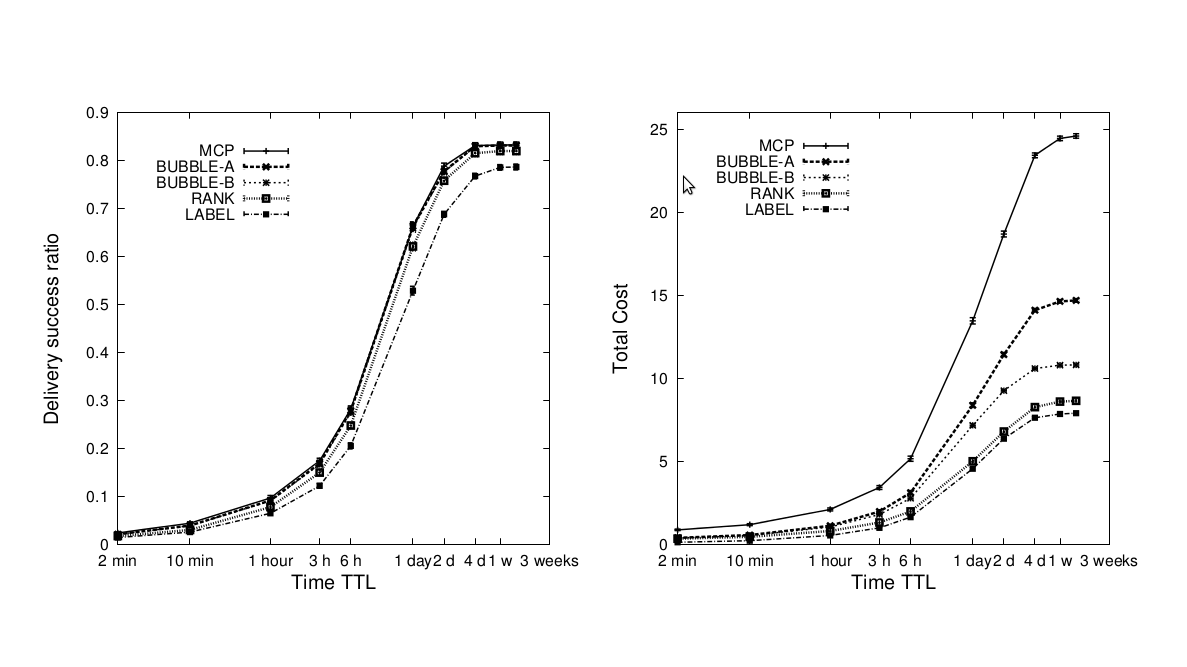
\includegraphics[scale=0.35]{img/bubblerap-performance.png}
    \caption{Compairson of several algorithms in two-community experiment based on \emph{Haggle Project} data sets}
  \end{center}
\end{figure}


\newpage
\newpage
\section{The Experiment}
\label{experiment}

The goal of this section is to explain the experiment with all technical detail needed, from adopted models to results through scenarios and measures.\\
First of all experiment aims to measure efficiency of several forwarding algorithm in an infrastructure free scenario, where mobile nodes are able to interact with others only in a limited local area around them. \\
We measure forwarding algorithm performance in terms of:
\begin{list}{}
\item \emph{Delivery ratio}: $ \dfrac{Number Of Messages Delivered}{ Number Of Messages Sent } $ 
\item \emph{Delivery cost}:  $ \dfrac{Number Of Inflight Messages }{ Number Of Messages Sent } $
\end{list}
Delivery ratio could range from $0$ to $1$, and we are interested in the maximum delivery ratio value obtained through all simulation time. We care about maximum value in the all time span because we are simulating an opportunistic delay tolerant network. For delivery cost we consider it's maximum value (cost peek), it's average value and it's variance across the simulation time, and its correlation with delivery ratio.\\ 

\subsection{Models and algorithms}
\label{exp_incarnation}
Since experiment needs to simulate a realistic contact network dynamics, we based our simulation on the community based mobility model introduced in section\ref{mobility_community_based_model} which is able to reproduce credible human-like interaction traces. In order to use this tool we had to generate a social-network to feed the mobility model algorithm.\\
For this reason we choose to adopt the caveman enhanced network model described in section\ref{sn_caveman_model} where community structures are first class concept.\\
Also we implement a subset of the forwarding algorithm described in\ref{forwarding}, both social-based and non-social ones; in detail we ran experiment with the following forwarding algorithms:
\begin{itemize}
\item \emph{Flood}, which is the most effective algorithm (but also the most expensive in terms of message copies)
\item \emph{Label}, which exploit node's interests and consequential community patterns.
\item \emph{Rank}, where nodes popularity lead forwarding decisions.
\item \emph{Bubble}, where both node's interest and popularity are exploited according to algorithm\ref{r_bubble_alg}.
\end{itemize}

\subsection{Simulation platform}
\label{exp_platform}

We decide to use a simulation platform that lessen the abstraction gap between the conceptual space of our experiment and the platform abstractions. In detail our experiment mainly involves two main concepts: mobile nodes and social networks.\\
Since we think supporting mobility simulation is generally harder than supporting social network simulations we choose to adopt the \emph{Alchemist} simulation platform\cite{pianini-jos2013} because it has been explicitly designed to handle nodes mobility and contact networks.\\
A part of the class project work has been allocated in the extension of the Alchemist platform in order to: 
\begin{itemize}
\item Integrate the concept of social network and enable simulation on arbitrary topologies.
\item Design a mechanism which permit to define arbitrary network formation algorithm (aka auto-linking rule)\footnote{Alchemist use an auto-linking euclidean rule (based on euclidean distance) for determining when a mobile node has a neighbourhood relationship with another one}.
\item Support environment with multiple networking layers. For instance support an euclidean environment with mobile nodes that links each others based on their physical distance, and at the same time support the concept social neighbourhood, or in general another linking layer based on other - non euclidean - criteria.
\end{itemize}

With this extensions we are fully enabled to run the experiment described above, which exploits only a small part of the expressive power of this extension.\\
In fact adding a social networking conceptual space to alchemist's domain may enable simulations on social network formation and dynamics by simulating contacts and interactions between mobile nodes in several environmental conditions.\\

\subsubsection{Experiment set-up}
\label{exp_setup}

In order to obtain a significant statistical base we set-up 2 experimental session:
\begin{itemize}
\item First one composed by 100 runs for each forwarding algorithm with 60 mobile nodes\footnote{Datasets used for emulations in\cite{bubble} provide traces of a number of mobile devices between 40 and 100 units} distributed in 6 communities and 16 message to deliver (uniformly distributed across nodes population), each time with a randomized\footnote{We used the built-in Mersenne Twister algorithm provided by simulation platform} initial configuration in terms of relationship between mobile users and consequential contact traces.
\item Second one with the same characteristics of the previous except for the number of message to deliver: 100 per run. 
\end{itemize}
In these experiments we set-up all messages at configuration time, so every sender start delivering from the beginning of the simulation. This configuration make sense if we assume that the stochastic process we are simulating is ergodic, under this assumption we might consider the simulation as a valid time sample of the behaviour of the system under the specified load (in terms of message to deliver in a time span).\\
In figure \ref{fig:bubble_live_init} and \ref{fig:bubble_live} are represented environment and nodes in the simulation demo running on Alchemist.
\begin{figure}[h!]
	\begin{center}
    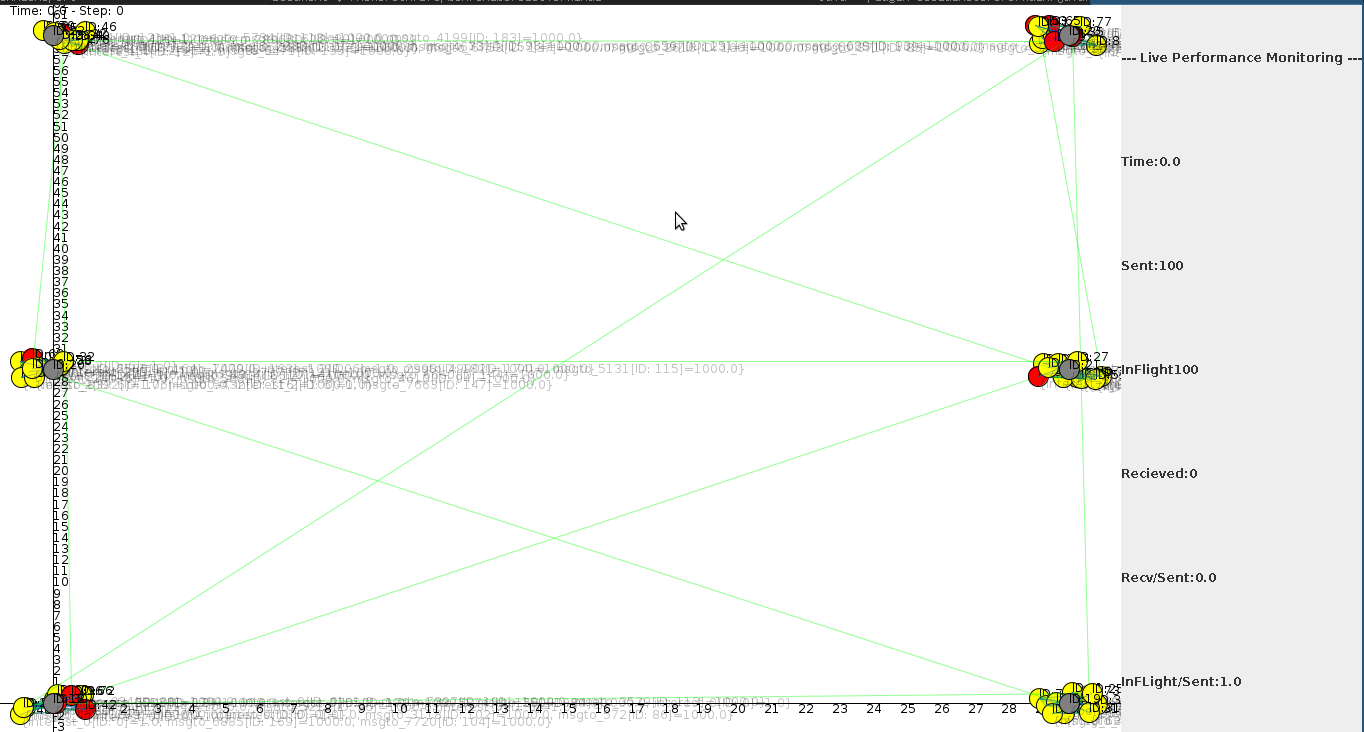
\includegraphics[scale=0.25]{img/bubble_live_init.png}
    \caption{Simulation initial configuration. Green lines represent social relationship while blue (shorter) lines physical links.}
    \label{fig:bubble_live_init}
  \end{center}
\end{figure}
\begin{figure}[h!]
	\begin{center}
    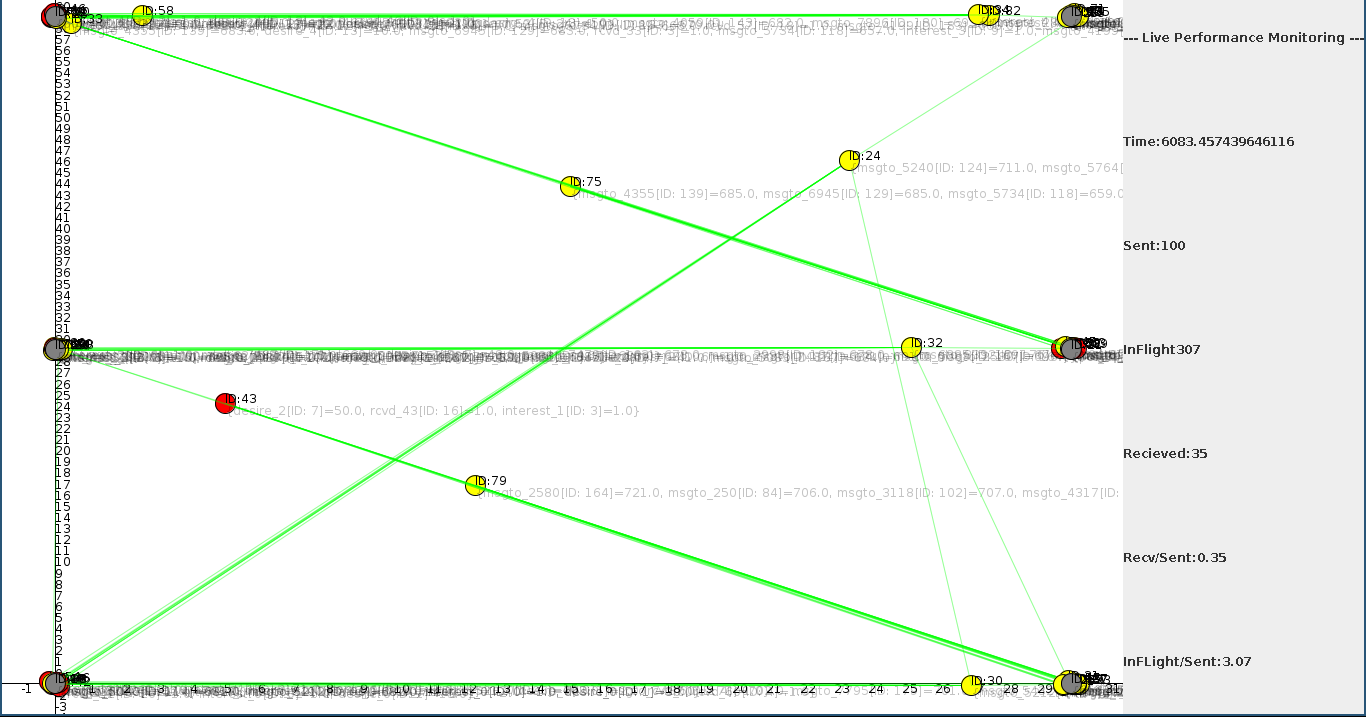
\includegraphics[scale=0.25]{img/bubble_live.png}
    \caption{Running simulation (bubble)}
    \label{fig:bubble_live}
  \end{center}
\end{figure}

\newpage
\subsubsection{Original Experiment}
In honour of completeness we briefly report emulation parameters and measurements reported in\cite[Table 3,6.2]{bubble}. The reference experiment - based on \emph{Reality data set} - involves 73 nodes subdivided in 8 communities (average size $\sim 9$) and a simulation time of 3 weeks. In figure \ref{fig:reality_emulation} are shown delivery ratio and cost measured during simulations.
\begin{center}
\begin{figure}[h!]
    		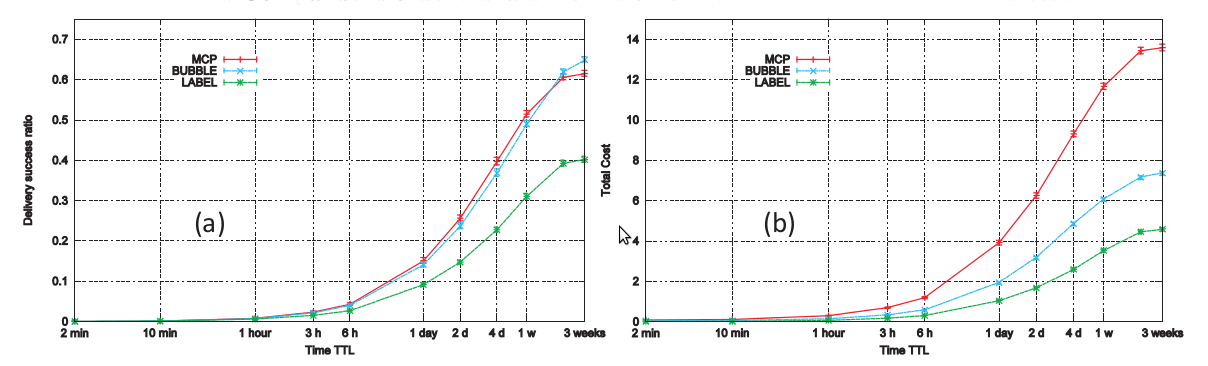
\includegraphics[scale=0.35]{img/reality_emulation.png}
    		\caption{Comparison of several algorithm performance reported in \cite{bubble} with \emph{Reality data set}. Figures \emph{a} and \emph{b} shows delivery ratio and cost respectively}
    		\label{fig:reality_emulation}
\end{figure}
\end{center}

\newpage
\subsection{Results}
\label{exp_results}

Simulation results have shown similar motifs with respect to emulation performed in\cite{bubble} and reported in figure\ref{fig:reality_emulation}, but values does not perfectly fit each others in term of absolute values. In fact we might note social based algorithm have lower delivery cost with respect to classical ones (eg. MCP in fig.\ref{fig:reality_emulation} and Flood in our experiments, fig.\ref{fig:run_1_aggregate}) and bubble algorithm has higher delivery ratio with respect to other social based algorithms.\\
The value difference could be caused by the load assumptions performed and the time span considered.\\
In fact in\cite[6.2]{bubble} time span considered is 3 week large ($1814400 sec$), with a presumable node velocity of $1\sim1.5 \frac{m}{sec^{-1}}$, instead simulated experiments range within 7 hours ($\sim 25000 sec$). So the 1000 message of the emulation are spread in a larger time span, with an average ratio of $5.5\cdot 10^{-4}$, while the 100 messages of the simulation are cumulated in a smaller time interval, with average ratio of $4\cdot 10^{-3}$. This mean a more stressed system.\\
Further simulation parameter tuning can be performed in order to refine experimental results: for example a finest set-up of nodes speed (and consequentially to the node movement reaction rate\footnote{Alchemist is based on chemical metaphor, so reactions (conditions and actions) happens with arbitrary rate}) or the rate of the moving decision's reactions should lead to more precise results. However results are also pretty interesting because reveal similar algorithms characteristics and led to the same efficiency conclusions.\\
Collected data of each experiment's run have been aggregated per time-interval, in other words we made an average of each runs measurement in each time sub-interval (one point on these graphs represent the average value measured for all the runs within the time interval considered). In addition we performed some classical statistic on un-aggregated data.\\
In figure ~\ref{fig:run_1_aggregate} ~\ref{fig:run_1_aggregate_noflood} and ~\ref{fig:run_2_aggregate} ~\ref{fig:run_2_aggregate_noflood} are represented delivery ratio and delivery cost of each algorithm during the simulation time (aggregated data).\\
\newpage
% Aggregated data session 1
\begin{center}
\begin{figure}[h!]
        \centering
    		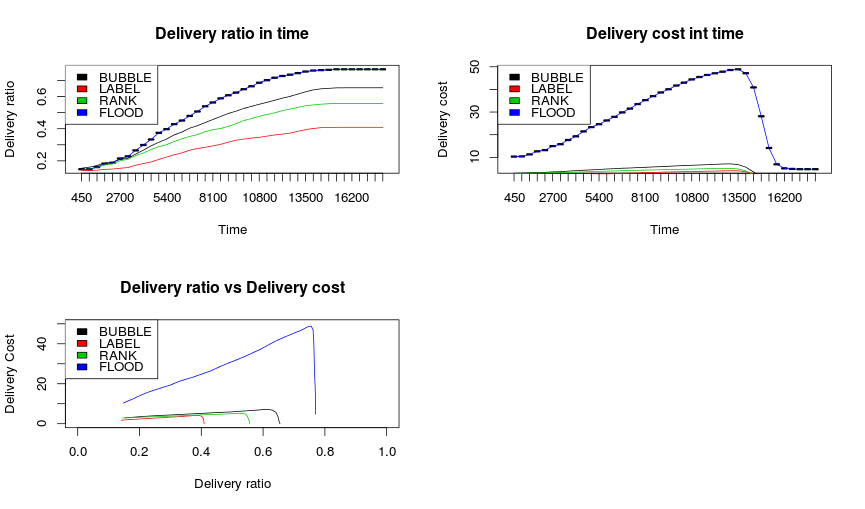
\includegraphics[scale=0.55]{img/run_1_aggregate.pdf}
    		\caption{Experimental session n.1 aggregated data}
    		\label{fig:run_1_aggregate}
\end{figure}
\begin{figure}[h!]
		\centering
    		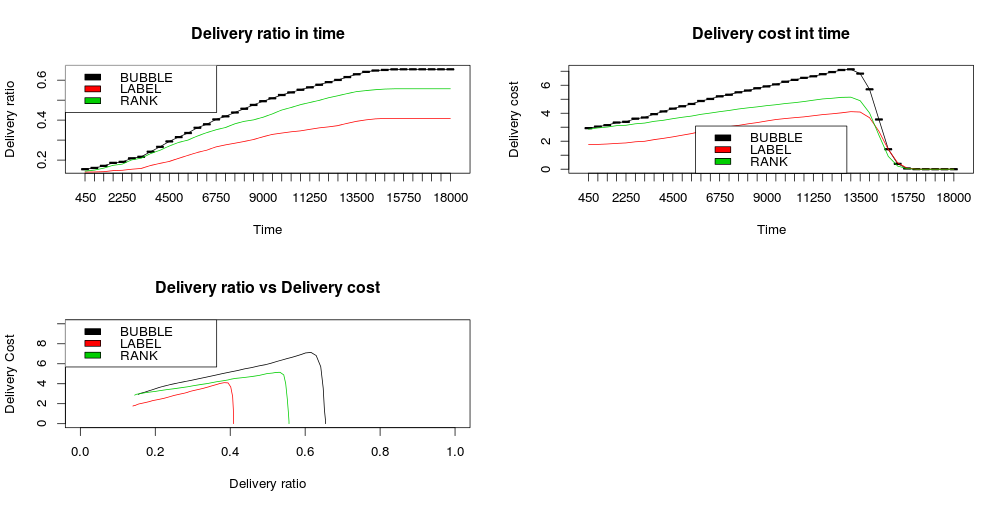
\includegraphics[scale=0.55]{img/run_1_aggregate_noflood.pdf}
    		\caption{Experimental session n.1 aggregated data without flood algorithm}
    		\label{fig:run_1_aggregate_noflood}
\end{figure}
\end{center}
\newpage
% Aggregated data session 2
\begin{figure}[h!]
	\begin{center}
    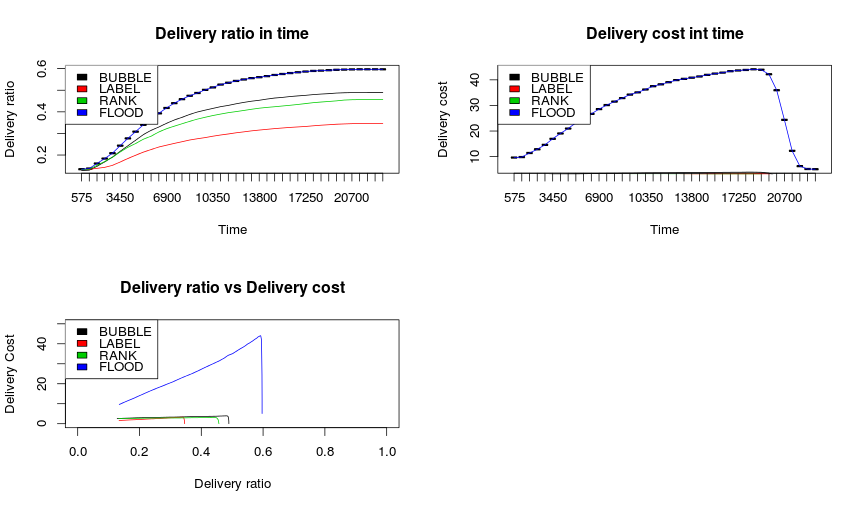
\includegraphics[scale=0.55]{img/run_2_aggregate.pdf}
    \caption{Experimental session n.2 aggregated data}
    \label{fig:run_2_aggregate}
  \end{center}
\end{figure}

\begin{figure}[h!]
	\begin{center}
    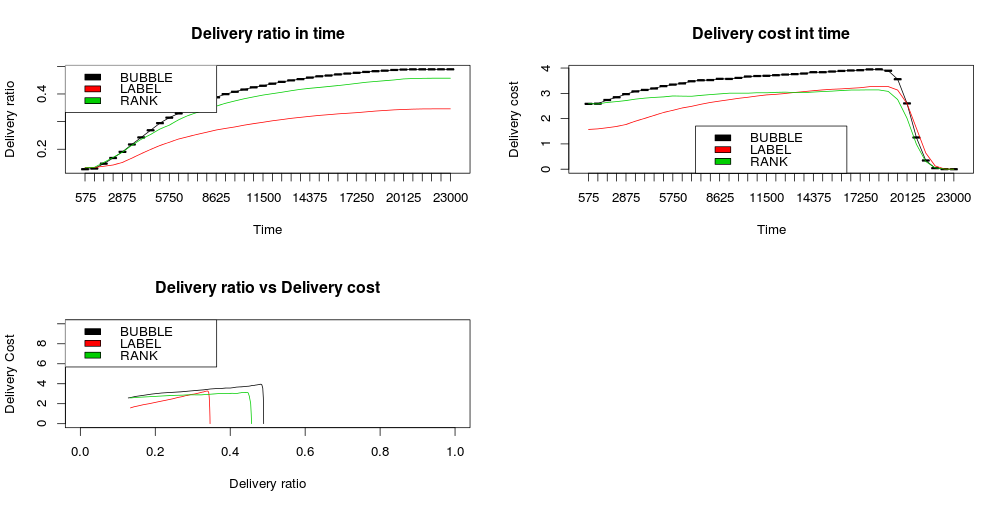
\includegraphics[scale=0.55]{img/run_2_aggregate_noflood.pdf}
    \caption{Experimental session n.2 aggregated data without flood algorithm}
    \label{fig:run_2_aggregate_noflood}
  \end{center}
\end{figure}
\newpage

While in figure ~\ref{fig:run_1_gstats} ~\ref{fig:run_2_gstats} are shown statistics about simulation session 1 and 2 subdivided per algorithm, and in ~\ref{fig:run_1_max_delratio} ~\ref{fig:run_2_max_delratio} are represented the distribution of the delivery ration across the runs.
% Statistics session 1
\begin{figure}[h!]
	\begin{center}
    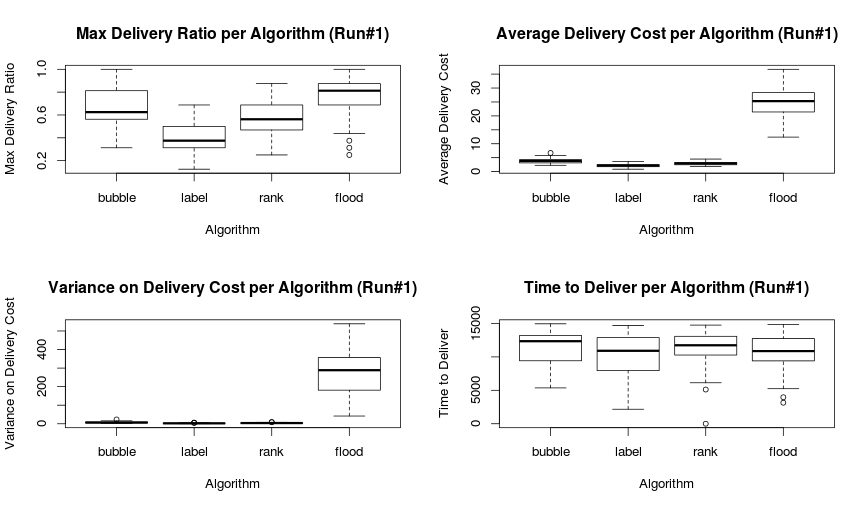
\includegraphics[scale=0.55]{img/run_1_gstats.pdf}
    \caption{Experimental session n.1 statistics}
    \label{fig:run_1_gstats}
  \end{center}
\end{figure}
% Statistics session 2
\begin{figure}[h!]
	\begin{center}
    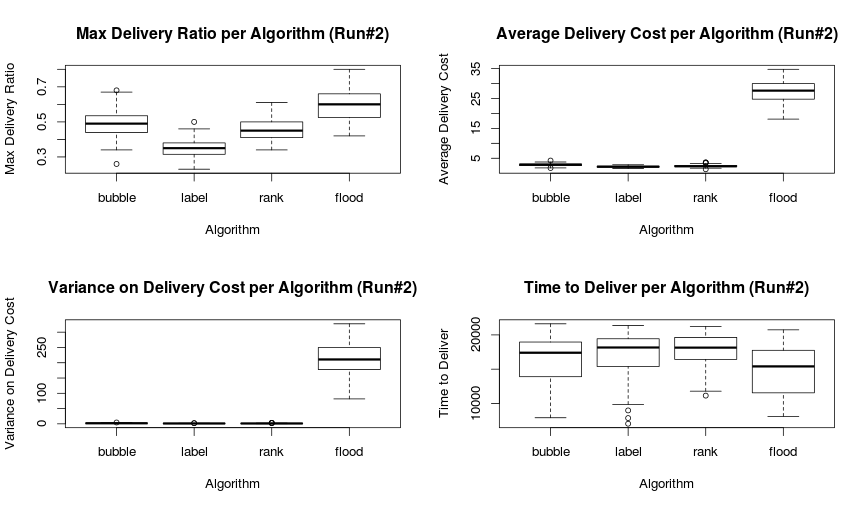
\includegraphics[scale=0.55]{img/run_2_gstats.pdf}
    \caption{Experimental session n.2 statistics}
    \label{fig:run_2_gstats}
  \end{center}
\end{figure}
\newpage
% Del ratio distribution session 1
\begin{figure}[h!]
	\begin{center}
    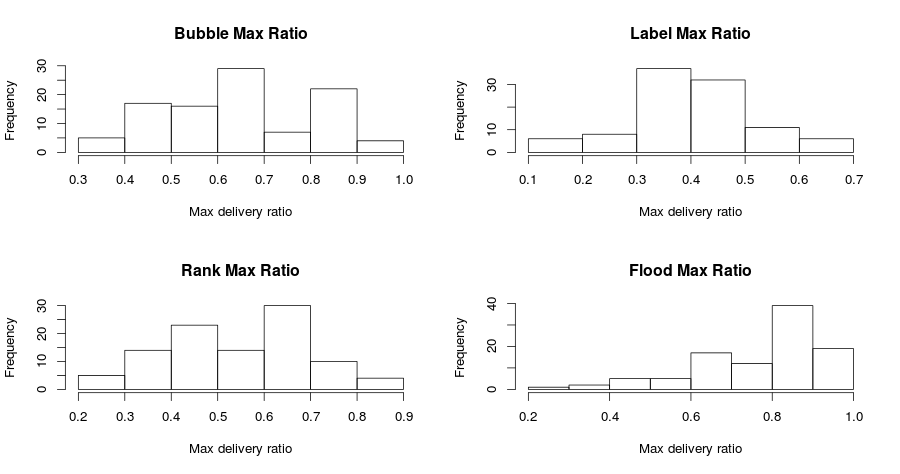
\includegraphics[scale=0.55]{img/run_1_max_delratio.pdf}
    \caption{Experimental session n.1 delivery ratio distribution}
    \label{fig:run_1_max_delratio}
  \end{center}
\end{figure}
% Del ratio distribution session 2
\begin{figure}[h!]
	\begin{center}
    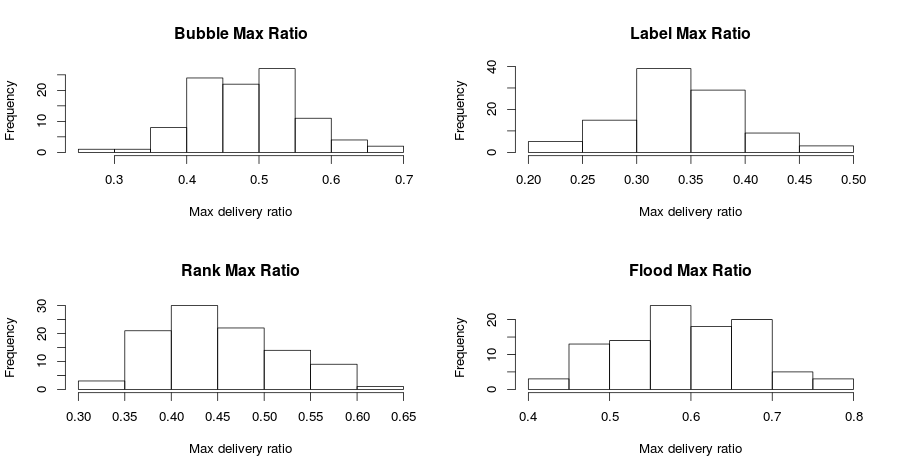
\includegraphics[scale=0.55]{img/run_2_max_delratio.pdf}
    \caption{Experimental session n.2 delivery ratio distribution}
    \label{fig:run_2_max_delratio}
  \end{center}
\end{figure}
\newpage

\newpage
\section{Conclusions}
\label{conclusions}

Despite the differences analyzed in \ref{exp_results}, we can derive same conclusion about algorithm efficiency: in fact flood algorithm results to be the upper bound in term of efficacy, label and rank algorithms have both lower cost w.r.t flood and also lower efficacy, instead bubble algorithm presents good delivered message/cost ratio, it also has comparable delivery delay with other algorithms.\\
This could indicate that this kind of simulations are a valid approach even in social based forwarding performance evaluation. Of course, as told before, further parameter refinement should be done in order to obtain more accurate measurements, and this could be valuable improvement in forwarding algorithm evaluation.\\
However the extensions developed on simulation platform (Alchemist) could also enable a new set of experimental scenarios: from social network formation to it's dynamics and maybe even the side effect on users mobility patterns. Naturally the limited amount of time available for class project are not enough for investigating the wide range of opportunities that the social network and mobility abstractions enable, so this class project could be considered as our first step into these topics.  


\newpage
\nocite{*}
\bibliography{biblio}{}
\bibliographystyle{plain} 

\newpage
\appendix
\appendixpage 
\section{Alchemist Repository}
Alchemist master branch is reachable at \url{https://bitbucket.org/danysk/alchemist}, while the extensions developed during class project ( \emph{incarnation-socialnets} and \emph{plugin-socialnets}) are publicly available at \url{https://bitbucket.org/lucam/alchemist}.
\section{Collected Data}
Experimental session data are also available at \url{TBD}. 
\section{Data Processing}
\lstinputlisting[label=r_script, language=R, breaklines=true, basicstyle=\tiny ,commentstyle=\color{mygreen},numbers=left,deletekeywords={var,time,col,max,path,*,\$,t,file,<\-}, numberstyle=\tiny\color{mygray}, caption=R Script used for data processing and visualization]{snippet/simstats.R}

\end{document}












